% Build with XeLaTeX or LuaLaTeX for robust fonts and math
\documentclass{article}

% Layout and packages
\usepackage[a4paper,margin=2.5cm]{geometry}
\usepackage{amsmath, amssymb, amsthm}
\usepackage{bm}
\usepackage{hyperref}
\usepackage{graphicx}
\usepackage{caption}
\usepackage{float} % For [H] placement
\usepackage{placeins}
\usepackage{listings}
\usepackage{xcolor}
\graphicspath{{figures/}}

% Code style
\lstdefinestyle{code}{
  basicstyle=\ttfamily\small,
  numbers=left,
  numberstyle=\tiny,
  numbersep=8pt,
  keywordstyle=\color{blue},
  commentstyle=\color{teal!70!black},
  stringstyle=\color{orange!70!black},
  showstringspaces=false,
  breaklines=true,
  frame=single,
  framerule=0.3pt,
  rulecolor=\color{black!15}
}
\lstset{style=code}

\title{Regularization Methods in Regression: Ridge, Lasso, and Elastic Net}
\author{}
\date{\today}

\begin{document}
\maketitle

\section{Introduction}
Regularization controls model complexity to mitigate overfitting and improve generalization. In linear regression, common methods are Ridge (\(\ell_2\)), Lasso (\(\ell_1\)), and Elastic Net (a mixture). They shrink coefficients toward zero, trading a bit of bias for reduced variance; Lasso additionally induces sparsity for embedded feature selection.

\section{Theory and Formulas}
\subsection{Model}
For features \(\mathbf{x} \in \mathbb{R}^d\): \(\hat{y} = \mathbf{w}^\top \mathbf{x} + b\). Intercept \(b\) is typically not penalized.

\subsection{Ridge (\(\ell_2\))}
\begin{equation}
\min_{\mathbf{w},b}\; \frac{1}{2n}\lVert \mathbf{X}\mathbf{w} + b\mathbf{1} - \mathbf{y} \rVert_2^2 + \frac{\lambda}{2} \lVert \mathbf{w} \rVert_2^2.
\end{equation}
Closed form (without penalizing intercept): \(\;\mathbf{w}^* = (\mathbf{X}^\top\mathbf{X} + \lambda \mathbf{I})^{-1}\mathbf{X}^\top(\mathbf{y}-\bar{y}\mathbf{1})\). Ridge shrinks coefficients continuously and handles multicollinearity but does not yield exact zeros.

\subsection{Lasso (\(\ell_1\))}
\begin{equation}
\min_{\mathbf{w},b}\; \frac{1}{2n}\lVert \mathbf{X}\mathbf{w} + b\mathbf{1} - \mathbf{y} \rVert_2^2 + \lambda \lVert \mathbf{w} \rVert_1.
\end{equation}
Encourages sparsity (some \(w_j=0\)). Subgradient/KKT conditions imply coefficients become zero when their correlation with residuals is within a \([-\lambda,\lambda]\) band.

\subsection{Elastic Net}
Combines \(\ell_1\) and \(\ell_2\):
\begin{equation}
\min_{\mathbf{w},b}\; \frac{1}{2n}\lVert \mathbf{X}\mathbf{w} + b\mathbf{1} - \mathbf{y} \rVert_2^2 + \lambda\left( \alpha \lVert \mathbf{w} \rVert_1 + \frac{1-\alpha}{2} \lVert \mathbf{w} \rVert_2^2 \right),\; \alpha\in[0,1].
\end{equation}
Useful with groups of correlated features: the \(\ell_2\) part stabilizes selection while \(\ell_1\) keeps sparsity.

\subsection{Standardization and Intercept}
Standardize feature columns and center \(\mathbf{y}\). Do not penalize \(b\); fit it on centered data.

\subsection{Optimization}
Ridge has a closed form or can be solved via QR/SVD. Lasso and Elastic Net are commonly optimized by coordinate descent using soft-thresholding with warm starts along a decreasing \(\lambda\) path.

\section{Applications and Tips}
\begin{itemize}
  \item \textbf{Multicollinearity}: Prefer Ridge or Elastic Net to stabilize estimates.
  \item \textbf{Feature selection}: Use Lasso/Elastic Net for sparsity and interpretability.
  \item \textbf{Model selection}: Tune \(\lambda\) (and \(\alpha\)) via cross-validation; inspect coefficient paths and validation curves.
  \item \textbf{Preprocessing}: Standardize features; remove or cap outliers; consider grouping correlated variables.
\end{itemize}

\section{Python Practice: Paths for Ridge and Lasso}
This example generates synthetic data, then plots coefficient paths for Lasso and Ridge across regularization strengths, saving to \texttt{figures/lasso\_path.png} and \texttt{figures/ridge\_path.png}.

\begin{lstlisting}[language=Python,caption={gen_regularization_figures.py}]
import os
import numpy as np
import matplotlib.pyplot as plt
from sklearn.linear_model import lasso_path, Ridge

np.random.seed(7)

n, d = 120, 12
X_raw = np.random.randn(n, d)
X_raw[:, 1] = 0.7*X_raw[:, 0] + 0.3*np.random.randn(n)

true_w = np.zeros(d)
true_w[[0, 3, 7]] = [2.0, -3.0, 1.5]
y = X_raw @ true_w + 0.8*np.random.randn(n)

# Standardize features and center y
X = (X_raw - X_raw.mean(axis=0)) / X_raw.std(axis=0)
y = y - y.mean()

# Lasso path (alphas descending); sklearn uses alpha=lambda/n_samples
alphas_lasso, coefs_lasso, _ = lasso_path(X, y, alphas=None)

fig, ax = plt.subplots(figsize=(7, 4.5))
for j in range(d):
    ax.plot(alphas_lasso, coefs_lasso[j, :], lw=1.6, label=f"w{j}")
ax.set_xscale('log'); ax.invert_xaxis()
ax.set_xlabel('alpha (log)'); ax.set_ylabel('coefficient')
ax.set_title('Lasso coefficient paths')
handles, labels = ax.get_legend_handles_labels()
ax.legend(handles[:6], labels[:6], loc='best', fontsize=8)

fig_dir = os.path.join(
    "0_Machine Learning", "0_Supervised Learning", "1_Regularization Methods in Regression", "figures")
os.makedirs(fig_dir, exist_ok=True)
plt.tight_layout(); plt.savefig(os.path.join(fig_dir, 'lasso_path.png'), dpi=160)

# Ridge path across a grid of alphas
alphas_ridge = np.logspace(-3, 2, 40)
coefs_ridge = []
for a in alphas_ridge:
    model = Ridge(alpha=a, fit_intercept=False)
    model.fit(X, y)
    coefs_ridge.append(model.coef_)
coefs_ridge = np.array(coefs_ridge)  # shape (len(alphas_ridge), d)

fig, ax = plt.subplots(figsize=(7, 4.5))
for j in range(d):
    ax.plot(alphas_ridge, coefs_ridge[:, j], lw=1.6, label=f"w{j}")
ax.set_xscale('log'); ax.invert_xaxis()
ax.set_xlabel('alpha (log)'); ax.set_ylabel('coefficient')
ax.set_title('Ridge coefficient paths')
handles, labels = ax.get_legend_handles_labels()
ax.legend(handles[:6], labels[:6], loc='best', fontsize=8)

plt.tight_layout(); plt.savefig(os.path.join(fig_dir, 'ridge_path.png'), dpi=160)
print('saved to', os.path.join(fig_dir, 'lasso_path.png'), 'and ridge_path.png')
\end{lstlisting}

\section{Result}
Figures~\ref{fig:lasso_path} and~\ref{fig:ridge_path} show how coefficients evolve with regularization strength. Lasso induces sparsity; Ridge shrinks continuously without zeros.

\begin{figure}[H]
  \centering
  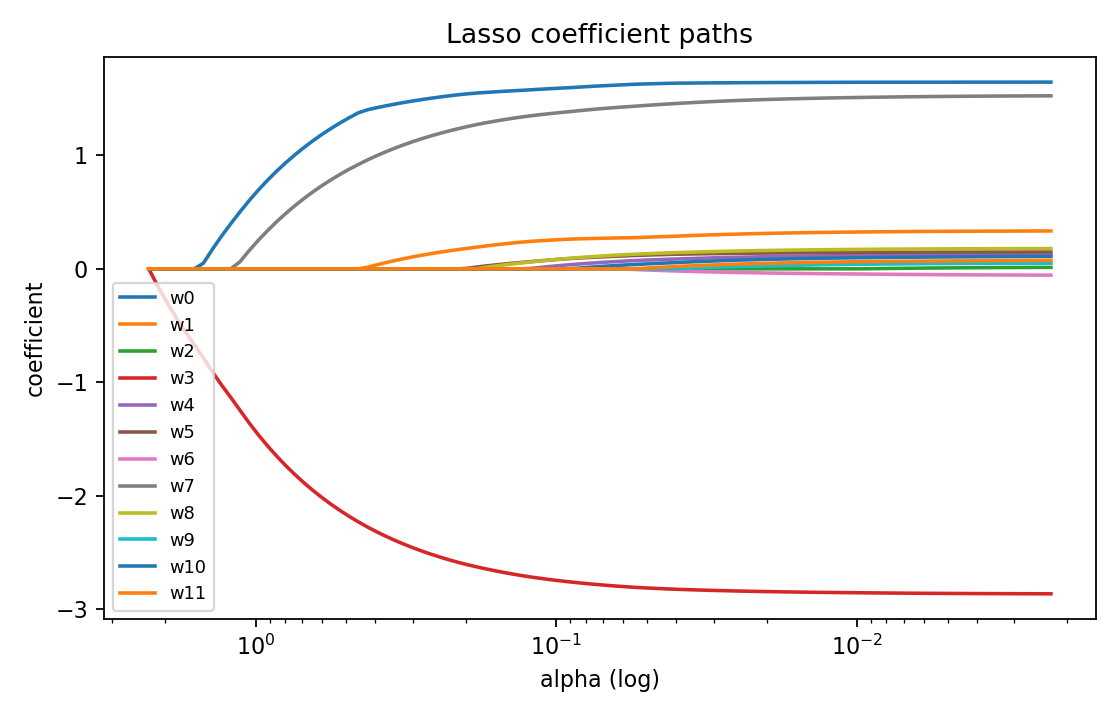
\includegraphics[width=0.85\linewidth]{lasso_path.png}
  \caption{Lasso coefficient paths on synthetic data}
  \label{fig:lasso_path}
\end{figure}

\begin{figure}[H]
  \centering
  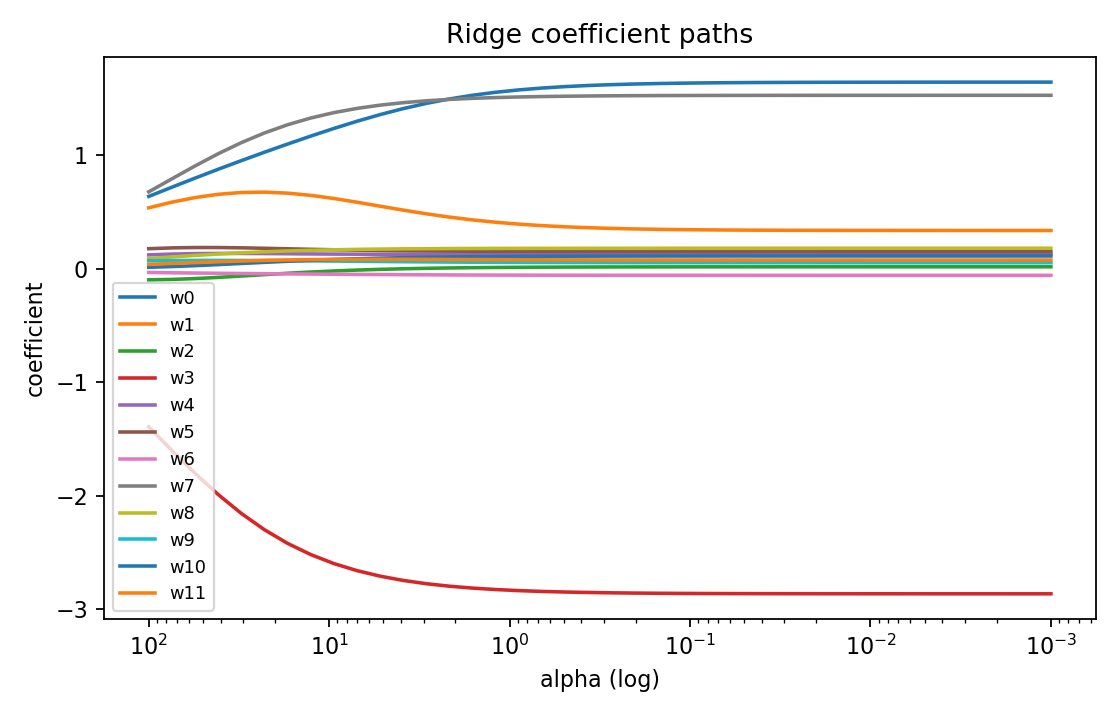
\includegraphics[width=0.85\linewidth]{ridge_path.png}
  \caption{Ridge coefficient paths on synthetic data}
  \label{fig:ridge_path}
\end{figure}

\FloatBarrier

\section{Summary}
Regularization manages variance and improves generalization. Use Ridge for stability under multicollinearity, Lasso for sparse, interpretable models, and Elastic Net when features are correlated. Always standardize features and select hyperparameters via cross-validation.

\end{document}
